\documentclass[darktitle]{beamer}
\usepackage{caption}
\usepackage{color}
\usepackage{graphicx}

\usepackage{color}
\definecolor{dkgreen}{rgb}{0,0.6,0}
\definecolor{gray}{rgb}{0.5,0.5,0.5}
\definecolor{mauve}{rgb}{0.58,0,0.82}
\definecolor{javared}{rgb}{0.6,0,0} % for strings
\definecolor{javagreen}{rgb}{0.25,0.5,0.35} % comments
\definecolor{javapurple}{rgb}{0.5,0,0.35} % keywords
\definecolor{javadocblue}{rgb}{0.25,0.35,0.75} % javadoc

\usepackage{listings}
\lstset{language=Java,
basicstyle=\ttfamily,
keywordstyle=\color{javapurple}\bfseries,
stringstyle=\color{javared},
commentstyle=\color{javagreen},
morecomment=[s][\color{javadocblue}]{/**}{*/},
numbers=left,
numberstyle=\tiny\color{black},
stepnumber=2,
numbersep=10pt,
	xleftmargin=15pt,
	xrightmargin=15pt,
	breaklines=true,
	frame=l,
tabsize=4,
showspaces=false,
showstringspaces=false,
basicstyle=\ttfamily\scriptsize}
%\lstloadlanguages{{XML}}

\lstset{lan­guage=Java}

\DeclareCaptionFormat{plain}{#3}

\usetheme{QE}


\title{AndroidTracker}
\author{Christoph Leitner, Alexandra J\"ager}
%\mail{\{c.leitner, alexandra.jaeger\}@student.uibk.ac.at}
\date{\today}

\begin{document}

	\begin{frame}
		\titlepage
	\end{frame}

	\begin{frame}
		\frametitle{Task}
		\begin{itemize}
			\item Write an Android application that tracks a user
			\item Runs in background
			\item Sends GPS location information to Web application
			\item Uses Wifi to determine location of the device
			\item Allow remote locking of the device
			\item Build a Web application that plots the user's activity
		\end{itemize}
	\end{frame}

	\begin{frame}
		\frametitle{App}
		\begin{itemize}
			\item built for Android 4.3
			\item use Google Play Services to read GPS data from mobile phone
			\item use HTTP-POST to send it to server
			\item information sent:
				\begin{itemize}
					\item IMEI -- unique device identification
					\item LAT -- GPS coordinates: latitude
					\item LONG -- GPS coordinates: longitude
				\end{itemize}
		\end{itemize}
		
	\end{frame}

	\begin{frame}
		\frametitle{Web Application}
		\begin{itemize}
			\item use XAMPP to set up a local server
			\item you can register a username to an IMEI
			\item use username or IMEI to "log in" to only see the locations associated with your IMEI  (username is just an alias for the IMEI -- locations are also tracked without registration)
			\item locations are displayed using Google Map Markers
			\item numbers are written in the markers to indicate the order in which the location data has been received
		\end{itemize}
	\end{frame}

	\begin{frame}
		\frametitle{Web Application - Screenshot}
		\begin{center}
		\includegraphics[height=0.75\textheight]{figures/webApp_screenshot.pdf}
		\end{center}
	\end{frame}

	\begin{frame}
		\frametitle{TODOs}
		\begin{itemize}
			\item Remote locking
			\item HTTPS
			\item improved user management (passwords!)
			\item improved user interface
		\end{itemize}
	\end{frame}

	\begin{frame}
		\frametitle{Thank you for your attention!}
		\begin{itemize}
			\item[] \huge{QUESTIONS?}
		\end{itemize}
	\end{frame}

	
\end{document}
